\documentclass[10pt,a4paper]{article}

\usepackage[utf8]{inputenc}
\usepackage[LGR,T1]{fontenc}
\usepackage[greek,english]{babel}
\usepackage[english]{isodate}
\usepackage[parfill]{parskip}
\usepackage{graphicx}
\usepackage{pdfpages}
\usepackage{setspace}
\usepackage{amsmath}
\usepackage{listings}
\usepackage{color}
\usepackage{fancyhdr}
\usepackage{hyperref}
\hypersetup{
    colorlinks=true,
    linktoc=all,
    linkcolor=black,
}
\lstdefinestyle{mystyle}{
backgroundcolor=\color{backcolour},
commentstyle=\color{codegreen},
keywordstyle=\color{magenta},
numberstyle=\tiny\color{codegray},
stringstyle=\color{codepurple},
basicstyle=\tiny,
breakatwhitespace=false,
breaklines=true,
captionpos=b,
keepspaces=true,
numbers=left,
numbersep=5pt,
showspaces=false,
showstringspaces=false,
showtabs=false,
tabsize=2
}
\lstdefinestyle{secondStyle}{
backgroundcolor=\color{backcolour},
commentstyle=\color{codegreen},
keywordstyle=\color{magenta},
basicstyle=\footnotesize,
showspaces=false,
showstringspaces=false,
showtabs=false,
tabsize=2
}

\title{%
  \huge \textgreek{Ανάκτηση Πληροφορίας} \\
\large biznasearch - \textgreek{Μηχανή αναζήτησης επιχειρήσεων}}
\author{
    \textgreek{Δημήτριος Ν. Κουβέρης} (2730) \\
    \textgreek{Αλβάρο Α. Χύσι} (2574)
}
\date{\textgreek{Απρίλιος} 2019}

\definecolor{codegreen}{rgb}{0,0.6,0}
\definecolor{codegray}{rgb}{0.5,0.5,0.5}
\definecolor{codepurple}{rgb}{0.58,0,0.82}
\definecolor{backcolour}{rgb}{0.95,0.95,0.92}

\begin{document}

    % cover page
    \pagenumbering{gobble}

    \title{
    \huge \textgreek {Τελική Αναφορά - Οδηγείες Χρήσης}}

    \maketitle
    \newpage
    \renewcommand{\contentsname}{\textgreek{Περιεχόμενα}}
    \tableofcontents

    \pagenumbering{arabic}

    % introduction
    \newpage
    \section{\textgreek{Εισαγωγή}}
    \paragraph {\textgreek{Σκοπός.}}
\textgreek{Σκοπός της συγκεκριμένης εργασίας είναι η δημιουργία μίας μηχανής
ανάκτησης πληροφορίας. Συγκεκριμένα μια μηχανή αναζήτησης επιχειρήσεων
με την χρήση της βιβλιοθήκης $Lucene$.}

\paragraph{Dataset.}
\textgreek {
    Χρησιμοποιήθηκε η συλλογή δεδομένων από το }
    Yelp. \\ https://www.yelp.com/dataset/challenge.
\textgreek{
    Μια συλλογή από εκατοντάδες χιλιάδες επιχειρήσεις και μερικών εκατομμυρίων
    σχολίων και υποδείξεων για αυτές.
}

\paragraph{\textgreek{Στόχοι - Απαιτούμενα}}
\begin{enumerate}
    \item \textgreek{Ανάλυση και κατασκευή ευρετηρίου}
    \item \textgreek{Αναζήτηση}
        \begin{itemize}
            \item \textgreek {Με βάση το όνομα της επιχείρησης}
            \item \textgreek {Με βάση τις κατηγορίες της επιχείρησης}
            \item \textgreek {Με βάση φράσεις - λέξεις κλειδιά}
            \item \textgreek {Σύνθετες δυαδικές ερωτήσεις ($boolean queries$)}
        \end{itemize}
    \item \textgreek{Διάταξη}
        \begin{itemize}
            \item \textgreek{Αναδιάταξη με βάση τα αστέρια κάθε επιχείρησης}
            \item \textgreek{Αναδιάταξη με βάση το πλήθος των κριτικών της κάθε επιχείρησης}
        \end{itemize}
    \item Misc
        \begin{itemize}
            \item Query Result Highlighting
        \end{itemize}
    \item {Bonus Functionality}
        \begin{itemize}
            \item FAQs
            \item\textgreek{Αναδιάταξη με βάση το πλήθος κλικ προηγούμενων αναζητήσεων}
            \item\textgreek{Αναδιάταξη με βάση το ιστορικό αναζητήσεων}
            \item\textgreek{Πρόταση δημοφιλών ερωτήσεων}
        \end{itemize}
\end{enumerate}


    % data processing
    \section{\textgreek{Προεπεξεργασία Δεδομένων}}
    \subsection{\textgreek {Επεξεργασία συλλογής}}
\textgreek{
    Η αρχική μορφή των δεδομένων ήταν τύπου $json$.
    Τα δεδομένα μετατράπηκαν
    σε μορφή τύπου $csv$, με σκοπό την ταχύτερη εισαγωγή τους στη βάση δεδομένων.

    Για τη μετατροπή χρησιμοποιήθηκε το πρόγραμμα $jq$.
    Το $script$ για την
    \\ μετατροπή είναι το $src/main/resources/json\_to\_csv.sh$
}
\lstset{
basicstyle=\footnotesize,
showstringspaces=false,
commentstyle=\color{red},
keywordstyle=\color{blue},
breakatwhitespace=false,
breaklines=true
}
\begin{lstlisting}[language=bash]
    #!/bin/bash

    # example usage of `jq` for exporting to tsv
    jq -r '[.business_id, .name, .latitude, .longitude, .city, .stars, .review_count, .address, .postal_code, .categories] | @tsv' \
    business.json                               \
    | tr "\"" "'"                               \
    > businesses.tsv

    jq -r '[.review_id, .business_id, .stars, .date, .text, .useful, .funny, .cool] | @tsv' \
    review.json                               \
    | tr "\"" "'"                               \
    > reviews.tsv

    jq -r '[.text, .date, .compliment_count, .business_id] | @tsv' \
    tip.json                               \
    | tr "\"" "'"                               \
    > tips.tsv

\end{lstlisting}


\subsection{\textgreek{Βάση Δεδομένων}}
\textgreek{
    Με στόχο την καλύτερη και ευκολότερη διαχείρηση των δεδομένων σε μια
    πιο δομημένη μορφή, δημιουργήθηκε σχεσιακή βάση δεδομένων.

    Το σύστημα διαχείρησης της βάσης δεδομένων που χρησιμοποιήθηκε
    είναι $Postgres$. Το σχήμα που δημιουργήθηκε φαίνεται παρακάτω.

\begin{center}
    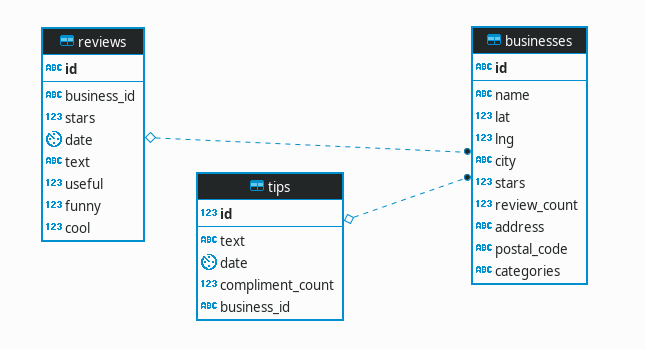
\includegraphics[width=130mm]{media/schema.png}
\end{center}
}

\subsection{\textgreek{Στατιστικά δεδομένων}}
    \textgreek{
    Μετά την εισαγωγή των δεδομένων στην βάση μας,
    με κατάλληλα ερωτήματα $SQL$ μπορούμε να βγάλουμε χρήσιμα στατιστικά
    προκειμένου να γίνει καλύτερη κατανόηση των δεδομένων μας.
    }

    \paragraph{\textgreek{Στατιστικά πόλεων}}
    \textgreek{
        Παρακάτω φαίνονται μερικά χρήσιμα στατιστικά ανα πόλη.

    \begin{enumerate}
        \item \textgreek{Αριθμός επιχειρήσεων ανά πόλη.}
        \item \textgreek{Αριθμός κριτικών ανά πόλη.}
        \item \textgreek{Μέσος αριθμός κριτικών και υποδείξεων.}
        \item \textgreek{Αριθμός υποδείξεων ($tips$) ανά πόλη.}
    \end{enumerate}

    \begin{center}
        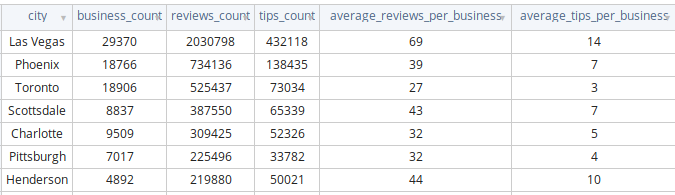
\includegraphics[width=130mm]{media/stats_table.png}
        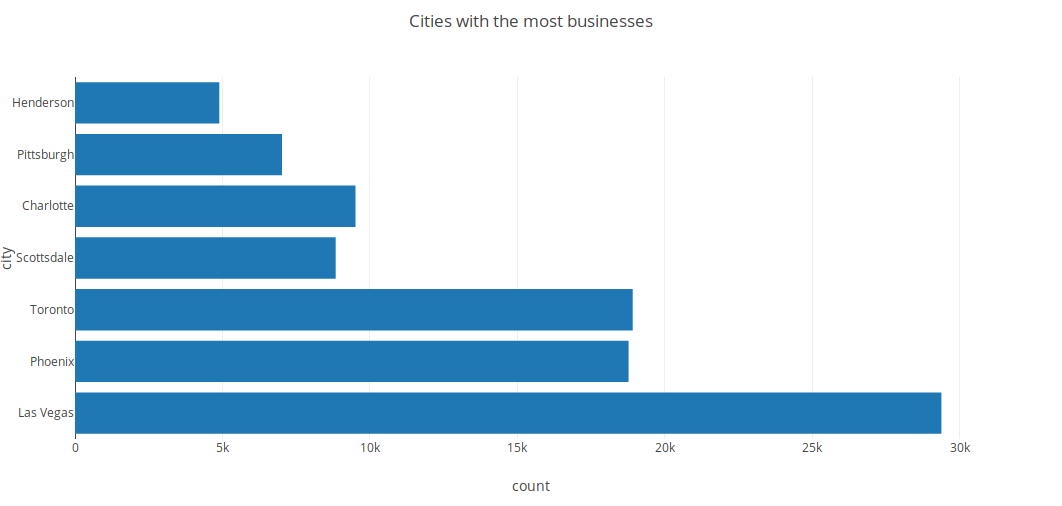
\includegraphics[width=130mm]{media/business_count_chart.png}
        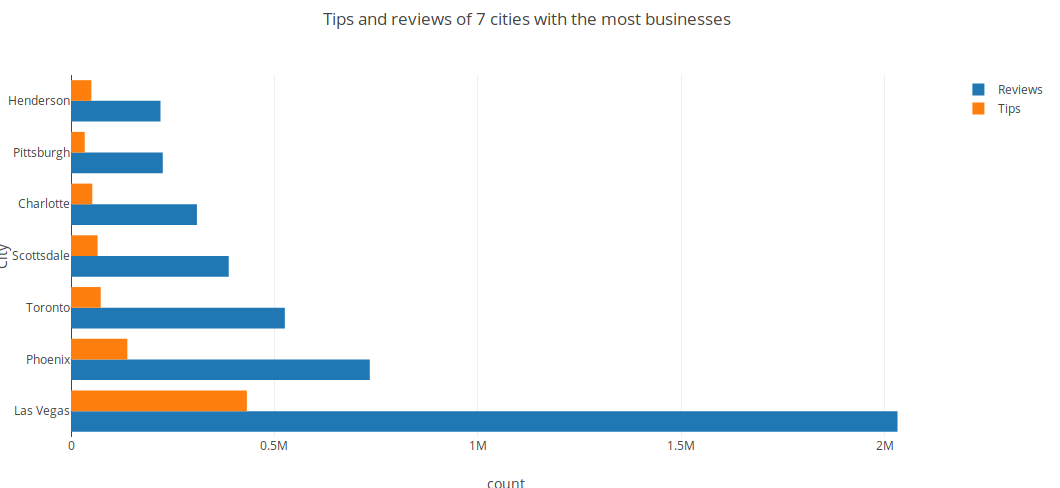
\includegraphics[width=130mm]{media/reviews_and_tips_chart.png}
    \end{center}

    \textgreek{
    Συνεπώς με βάση και με τα παραπάνω σχήματα επιλέξαμε την πόλη του $Las$ $Vegas$
    ως την πόλη πάνω στην οποία θα χτίσουμε την μηχανή αναζήτησής μας. Συγκεκριμένα
    έχει 29,400 επιχειρήσεις και συνολικα 2,470,000 κριτικές και υποδείξεις.
    }
}


    % app schema
    \section{\textgreek{Σχήμα Εφαρμογής}}
    \textgreek {

Η εφαρμογή μας δουλεύει με βάση έναν διακομιστή ο οποίος επικοινωνεί με την βάση δεδομένων μας, τα αρχεία της $Lucene$
και το γραφικό περιβάλλον $html$.
Συγκεκριμένα όπως φαίνεται από το σχήμα, ο διακομιστής δέχεται αιτήματα απο τον χρήστη και επιστρέφει τις κατάλληλες
απαντήσεις. Ανάλογα με το αίτημα καλεί τις κατάλληλες μεθόδους της $lucene$ οι οποίες είτε επιστρέφουν αποτελέσματα αναζήτησης
στον διακομιστή ή δημιουργούν τα ευρετήρια αναζήτησης. Τέλος, ο διακομιστής επικοινωνεί με την βάση για να προσπελάσει τα στοιχεία που
επέστρεψε η αναζήτηση και να ανανεώσει το πεδίο $click$ της κάθε επιχείρησης.
}


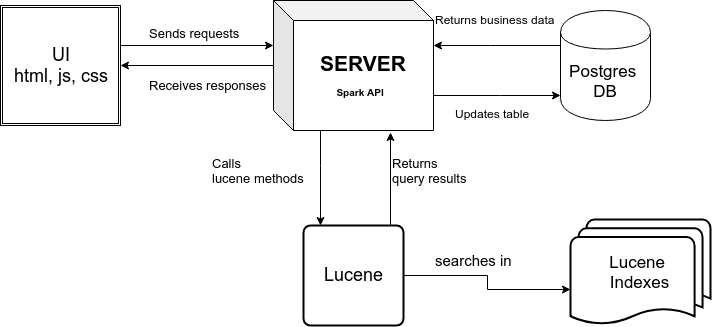
\includegraphics[width=1\textwidth]{media/app_schema.png}


    \section{\textgreek{Ευρετηριοποίηση}}
    

\lstset{style=mystyle}

\subsection{\textgreek{Δημιουργία ευρετηρίων}}
\paragraph{\textgreek{Έγγραφα}}\textgreek{
Χρησιμοποιήσαμε τις μεθόδους της $lucene$ για την δημιουργία των εγγράφων.
Συγκεκριμένα ένα εγγράφο για κάθε επιχείρηση με πεδία, $business\_id$, $business\_name$, $business\_categories$,
$review\_id$, $review\_text$, $tip\_id$, $tip\_text$.
Δηλαδή σε κάθε έγγραφο αποθηκεύουμε όλη την πληροφορία που θα χρειαστούμε για κάθε επιχείρηση.
}

\begin{lstlisting}[language=Java]

private void createBusinessIndex(String city) throws SQLException, IOException {
    Document docEntry;
    Path path = Paths.get(indexDir, "businesses");
    Directory businessIndex = FSDirectory.open(path);
    IndexWriterConfig indexWriterConfig = new IndexWriterConfig(analyzer);
    indexWriterConfig.setOpenMode(IndexWriterConfig.OpenMode.CREATE);
    IndexWriter indexWriter = new IndexWriter(businessIndex, indexWriterConfig);

    String sqlQuery = sqlBusinessesIdxColsOfCity(city);
    List<String> columns = Arrays.asList("id", "name", "categories");

    PreparedStatement pst = dbConnection.prepareStatement(sqlQuery);
    pst.setFetchSize(100);
    ResultSet rs = pst.executeQuery();

    long startTime = System.currentTimeMillis();
    int cnt = 0;

    System.out.println(">>> Starting indexing");
    while (rs.next()) {
        docEntry = new Document();
        for (int i = 0; i < columns.size(); i++) {
            docEntry.add(new Field(columns.get(i), rs.getString(i + 1), TextField.TYPE_STORED));
        }

        String sqlReviews = Shortcuts.sqlReviewsIdxColsWhereBusinessIdIs(rs.getString(1));
        PreparedStatement pstRevs = dbConnection.prepareStatement(sqlReviews);
        pstRevs.setFetchSize(100);
        ResultSet rsRevs = pstRevs.executeQuery();
        while (rsRevs.next()) {
            docEntry.add(new Field("review_id", rsRevs.getString(1), TextField.TYPE_STORED));
            docEntry.add(new Field("review", rsRevs.getString(2), TextField.TYPE_STORED));
        }

        String sqlTips = Shortcuts.sqlTipsIdxColsWhereBusinessIdIs(rs.getString(1));
        PreparedStatement pstTips = dbConnection.prepareStatement(sqlTips);
        pstTips.setFetchSize(100);
        ResultSet rsTips = pstTips.executeQuery();
        while (rsTips.next()) {
            docEntry.add(new Field("tip_id", rsTips.getString(1), TextField.TYPE_STORED));
            docEntry.add(new Field("tip", rsTips.getString(2), TextField.TYPE_STORED));
        }

        indexWriter.addDocument(docEntry);
        cnt++;

        if (cnt % 100 == 0) {
            double elapsedTimeSec = (System.currentTimeMillis() - startTime) / 1000.0;
            System.out.printf("\tindexed %d businesses in %.2fsec\n", cnt, elapsedTimeSec);
        }
    }

    indexWriter.close();
    double elapsedTimeSec = (System.currentTimeMillis() - startTime) / 1000.0;
    System.out.printf("\tindexed %d businesses in %.2fsec\n", cnt, elapsedTimeSec);

\end{lstlisting}

\textgreek{
Όπως βλέπουμε στο παραπάνω κομμάτι κώδικα, όταν ο χρήστης ζητήσει την δημιουργία ευρετηρίων στέλνουμε ένα αίτημα
στην βάση δεδομένων το οποίο μας επιστρέφει τις πληροφορίες που χρειαζόμαστε για την κάθε επιχείρηση. Σε κάθε επανάληψη
δημιουργούμε το εγγραφο και τα πεδία και τα εισάγουμε στη στο ευρετήριο μας με την εντολή
}
\lstset{style=secondStyle}
\begin{lstlisting}
indexWriter.addDocument(docEntry);
\end{lstlisting}

\subsection{SpellChecker}
\textgreek{
Υλοποιήσαμε την πρόβλεψη λέξεων και την διόρθωση λαθών. Χρησιμοποιήσαμε την κλάσση $Spellchecker$ της $lucene$ για να
δημιουργήσουμε ευρετήριο στο οποίο θα βρούμε τις πιο συναφείς λέξεις για να προτείνουμε στον χρήστη. Η συνάφεια
μετριέται με την χρήση της $Levenstein$ απόστασης.
}
\lstset{style=mystyle}
\begin{lstlisting}

\end{lstlisting}


    \section{\textgreek{Αναζήτηση}}
    \subsection{\textgreek{Επεξεργασία Ερωτημάτων}}
\textgreek {
    Ο διακομιστής στέλνει αίτημα αναζήτησης και καλεί την μέθοδο $search$ στο αρχείο $LuceneWrapper.java$.
    Η μέθοδος αυτή επεξεργάζεται το κείμενο του ερωτήματος και εντοπίζει αν είναι ερώτημα ενός ή πολλαπλών όρων.
    Αν είναι ένας όρος, κάνει αναζήτηση σε όλα τα πεδία του ευρετηρίου (δηλ. όνομα, κατηγορίες, κριτικές, υποδείξεις)
    δημιουργώντας έναν $multiFieldParser$.
    Αν πάλι το ερωτημά μας περιέχει ειδικούς χαρακτήρες και εντολές δημιουργείται $BooleanParser$ ή $PhraseParser$ για
    δυαδικές αναζητήσεις και αναζήτηση ολόκληρης φράσης, λέξης κλειδί αντίστοιχα.
    Η κλάσση $QueryParser$ επιτρέπει επίσης $wildcard$ αναζητήσεις και $term$ $boosting$.
}

\begin{lstlisting}[language=Java]
public List<SearchResult> search(String queryText, int resultsNum, String orderBy)
throws ParseException, SQLException, IOException, InvalidTokenOffsetsException {

    List<SearchResult> results = new ArrayList<>();
    List<String> fields = Arrays.asList("name", "categories", "review", "tip");
    QueryParser queryParser;
    IndexReader businessIndexReader = DirectoryReader.open(businessIndex);
    IndexSearcher searcher = new IndexSearcher(businessIndexReader);
    String[] querySplit = queryText.split(":");

    if (querySplit.length == 1) {
        queryText = querySplit[0];
        queryParser = new MultiFieldQueryParser(fields.toArray(new String[fields.size()]), analyzer);
    } else {
        if (!querySplit[1].matches("\\s+")) {
            querySplit[0] = querySplit[0].replaceAll("\\s+", "");
            if (!fields.contains(querySplit[0])) {
                queryText = "";
                for (String s : querySplit) {
                   queryText = queryText + " " + s;
                }
                queryText = queryText + "";
                queryParser = new MultiFieldQueryParser(fields.toArray(new String[fields.size()]), analyzer);
            } else {
                queryParser = new QueryParser(querySplit[0], new StandardAnalyzer());
            }
        } else {
            querySplit = queryText.replaceAll("\\s+", "").split(":");
            queryText = querySplit[0];
            queryParser = new MultiFieldQueryParser(fields.toArray(new String[fields.size()]), analyzer);
        }
    }

    Query query = queryParser.parse(queryText);
    System.out.println("Lucene Query: " + query.toString());

    TopDocs topDocs = searcher.search(query, resultsNum);
    List<String> businessIDs = new ArrayList<>();
    HashMap<String, String> businessHighlight = new HashMap<>();

    for (ScoreDoc top : topDocs.scoreDocs) {
        String businessID = searcher.doc(top.doc).get("id");
        String highlight = highLightQuery(query, top, queryParser.getField(), businessIndexReader, searcher);
        businessIDs.add(businessID);
        businessHighlight.put(businessID, highlight);
    }

    List<Business> businesses = Getters.businessesByIDs(dbConnection, businessIDs, orderBy);
    for (int i = 0; i < businesses.size(); i++) {
        Business business = businesses.get(i);
        String highlight = businessHighlight.get(business.getId());
        results.add(new SearchResult(business, highlight));
    }

    return results;
}

\end{lstlisting}

\subsection{\textgreek{Επιστροφή αποτελεσμάτων}}
\textgreek{
Τα $ids$ απο τα κορυφαία αποτελέσματα αποθηκεύονται σε μια λίστα αλφαριθμητικών, η οποία χρησιμοποιείται για να συνταχθεί
ενα $sql$ ερώτημα στην βάση μας και να επιστραφούν τα δεδομένα για την κάθε επιχείρηση.
}

\subsection{Highlighting}
\textgreek{
Με το πέρας της αναζήτησης χρησιμοποιούμε την κλάσση της $lucene$ $highlighter$ για να βρούμε και να
επισημάνουμε το κείμενο της αναζήτησης μας.
Η αναζήτηση αυτή επιστρέφει ένα $html formatted$ κείμενο, το οποίο το χρησιμοποιούμε στην προβολή των αποτελεσμάτων.
}

\subsection{\textgreek{Αναδιάταξη Αποτελεσμάτων}}
\textgreek{
Η μεθοδός μας παίρνει σαν παράμετρο τον τρόπο με τον οποίο θέλουμε να ταξινομήσουμε τα αποτελέσματά μας.
Η παράμετρος αυτή περνάει σαν όρισμα στην μέθοδο που συντάσσουμε το $sql$ ερώτημα και χρησιμοποιείται απο την βάση.
Η βάση αναδιατάσσει τα αποτελέσματα με βάση:
}
\begin{enumerate}
    \item\textgreek{ Με βάση τα αστέρια της κάθε επιχείρησης (με φθίνουσα ή αύξουσα σειρά)}
    \item\textgreek{ Με βάση το πλήθος των κριτικών της κάθε επιχείρησης (φθίνουσα ή αύξουσα σειρά)}
    \item\textgreek{ Με βάση το πλήθος των χρηστών που πάτησαν πάνω στην επιχείρηση σε προηγούμενες αναζητήσεις ($clickthrough$)}
    \item\textgreek{ Με βάση την προεπιλεγμένη κατάταξη της $lucene$ }
\end{enumerate}

\end{document}
